% Lecture Template for ME3001-001-Tristan Hill - Spring 2017 - Fall 2018
% 
% Mechanical Engineering Analysis with MATLAB
%



% Document settings
\documentclass[11pt]{article}
\usepackage[margin=1in]{geometry}
\usepackage[pdftex]{graphicx}
\usepackage{multirow}
\usepackage{setspace}
\usepackage{hyperref}
\usepackage{color,soul}
\usepackage{fancyvrb}
\usepackage{framed}
\usepackage{wasysym}
\usepackage{multicol}
%\usepackage{bigints}


\pagestyle{plain}
\setlength\parindent{0pt}
\hypersetup{
    bookmarks=true,         % show bookmarks bar?
    unicode=false,          % non-Latin characters in Acrobat’s bookmarks
    pdftoolbar=true,        % show Acrobat’s toolbar?
    pdfmenubar=true,        % show Acrobat’s menu?
    pdffitwindow=false,     % window fit to page when opened
    pdfstartview={FitH},    % fits the width of the page to the window
    pdftitle={My title},    % title
    pdfauthor={Author},     % author
    pdfsubject={Subject},   % subject of the document
    pdfcreator={Creator},   % creator of the document
    pdfproducer={Producer}, % producer of the document
    pdfkeywords={keyword1} {key2} {key3}, % list of keywords
    pdfnewwindow=true,      % links in new window
    colorlinks=true,       % false: boxed links; true: colored links
    linkcolor=red,          % color of internal links (change box color with linkbordercolor)
    citecolor=green,        % color of links to bibliography
    filecolor=magenta,      % color of file links
    urlcolor=blue           % color of external links
}

% assignment number 

\definecolor{mygreen}{rgb}{0, .39, 0}

%\definecolor{dred}{#8B0000}
% [153,50,204] - dark orchid
\definecolor{mypurple}{rgb}{0.6,0.1961,0.8}
%[139,69,19] - saddle brown
\definecolor{mybrown}{rgb}{0.5451,0.2706,0.0745}

\definecolor{mygray}{rgb}{.6, .6, .6}

\setulcolor{red} 
\setstcolor{green} 
\sethlcolor{mygray} 

\newcommand{\VA}{\vspace{2mm}}
\newcommand{\VB}{\vspace{5mm}} 
\newcommand{\VC}{\vspace{30mm}} 
 
\newcommand{\R}{\color{red}}
\newcommand{\B}{\color{blue}}
\newcommand{\K}{\color{black}}
\newcommand{\G}{\color{mygreen}}
\newcommand{\PR}{\color{mypurple}}

\newcommand{\NUM}{1} 
\newcommand{\VSpaceSize}{2mm} 
\newcommand{\HSpaceSize}{2mm} 

\begin{document}

\textbf{ \LARGE FE Review - Solid Mechanics - Dynamics} \\\\
\textbf{ \LARGE Review of Particle and Rigid Body Dynamics } \\
		
		\LARGE
		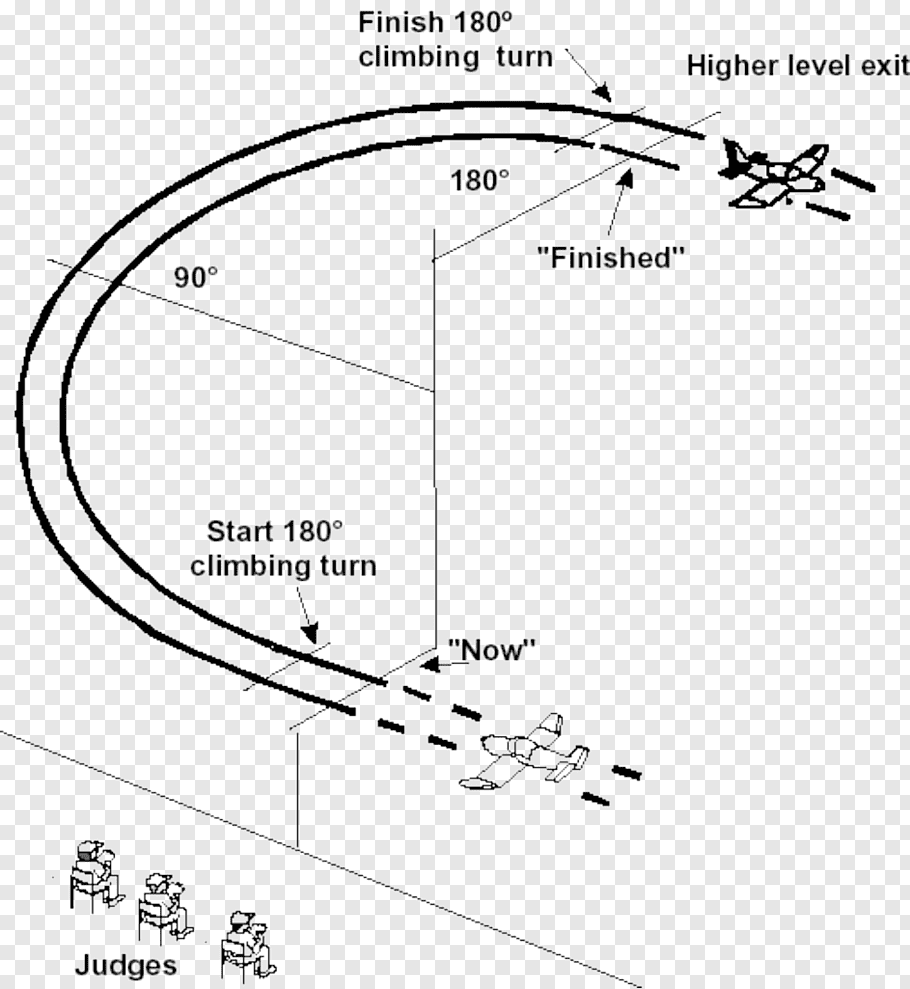
\includegraphics[scale=.25]{lecture1_fig1.png}\\
		\textbf{Outline:}\\
		
		\begin{itemize}
			\item Kinematics of a Particle
			\item Rigid Body Kinematics
			\item Newtons Laws of Motion
			\item Work and Energy Methods
			\item Kinetics of Rigid Bodies
		\end{itemize}


\newpage
		\begin{itemize}
			\item Kinematics of a Particle \\
		
			\scalebox{1.5}{$\vec{v}=\frac{d\vec{r}}{dt}=v\hat{e_t}$}  \vspace{2mm}\\

			\scalebox{1.5}{$\vec{a}=\frac{d\vec{v}}{dt}=\dot{v}\hat{e_t}+\vec{v}\frac{ds}{dt}\frac{d\hat{e_t}}{ds}=\dot{v}\hat{e_t}+\frac{\nu^2}{\rho}\hat{e_n}$}  \vspace{2mm}\\
		
			\scalebox{1.5}{$\frac{d\hat{e_t}}{ds}=\kappa \hat{e_n} $} \vspace{2mm}\\

			Distance Velocity and the Tangential Component of Acceleration \\

			\scalebox{1.5}{$\frac{d{v}}{dt}=a_t$} \hspace{10mm} or \hspace{10mm} \scalebox{1.5}{$v=v_0+\displaystyle\int a_tdt$}\vspace{2mm}\\\\
			\scalebox{1.5}{$\frac{d{s}}{dt}=v$} \hspace{10mm} or \hspace{10mm} \scalebox{1.5}{$s=s_0+\displaystyle\int vdt$}\\

			\scalebox{1.5}{$v\frac{dv}{ds}=a_t$} \hspace{10mm} or \hspace{10mm} \scalebox{1.5}{$v^2=v_0^2+2\displaystyle\int a_tds$} \\
			
			Constant Tangential Acceleration \\

			\scalebox{1.5}{$v=v_0+a_tt$} \vspace{2mm}\\
			
			\scalebox{1.5}{$s=s_0+v_0t+\frac{1}{2}a_tt^2$} \vspace{2mm}\\
	
			\scalebox{1.5}{$v^2=v_0^2+2a_ts$} \vspace{2mm}\\
	
\newpage
			\item Rigid Body Kinematics \\

			Constraint of Rigidity\\

			\scalebox{1.5}{$\frac{d}{dt}|r_{pq}|^2=\frac{d}{dt}(\vec{r}_{pq}\cdotp\vec{r}_{pq})=2\vec{r}_{pq}\cdotp\frac{d\vec{r}_{pq}}{dt}=0$} \vspace{2mm}\\

			Instantaneous Zero Velocity \\


			\item Newtons Laws of Motion \\

				\scalebox{1.5}{$\vec{f}=m\vec{a}$}\\

				\scalebox{1.5}{$\vec{p}=\displaystyle\Sigma_i m_iv_i$} \\\\

				\scalebox{1.5}{$\frac{d\vec{p}}{dt}=\displaystyle\Sigma_i m_ia_i$} \\\\

			\item Work and Energy Methods
			\item Kinetics of Rigid Bodies
		\end{itemize}
\newpage


\begin{itemize}
	\item  \textbf{\Large Example 8.8}: Piston, Crank and Connecting Rod\\


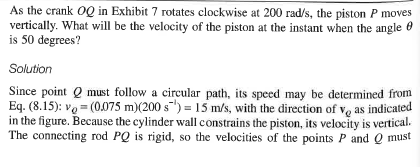
\includegraphics[scale=1.2]{example_8_8.png}
	
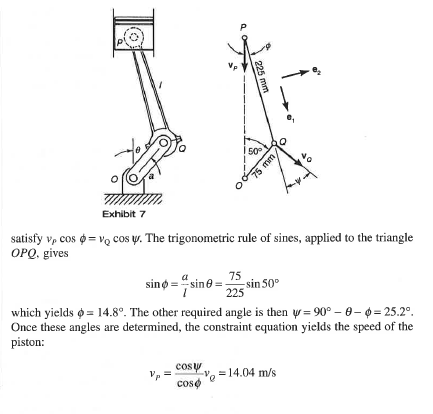
\includegraphics[scale=1.2]{example_8_8b.png}
	
\newpage
	\item  \textbf{\Large Example 8.9}: Piston, Crank and Connecting Rod\\

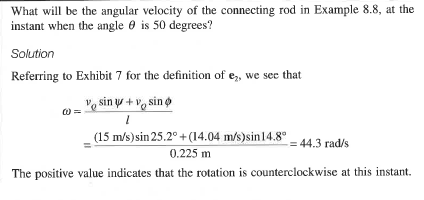
\includegraphics[scale=1.2]{example_8_9.png}


	
\newpage
	\item  \textbf{\Large Example 8.10}: Piston, Crank and Connecting Rod\\

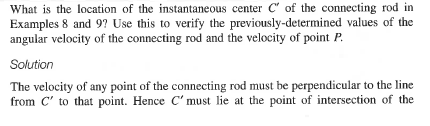
\includegraphics[scale=1.2]{example_8_10.png}

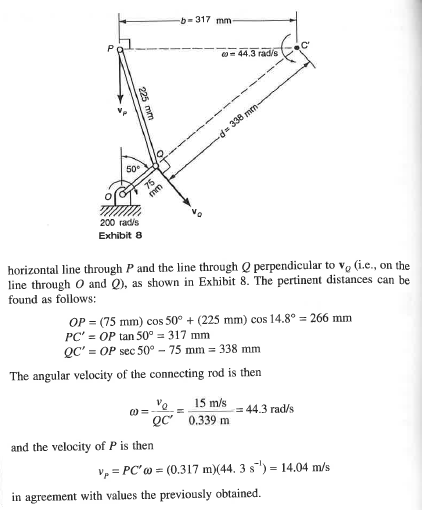
\includegraphics[scale=1.2]{example_8_10b.png}


\newpage
	\item  \textbf{\Large Example 8.12}: Piston, Crank and Connecting Rod\\

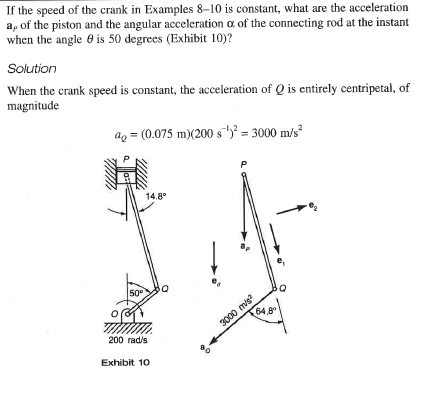
\includegraphics[scale=1.1]{example_8_12.png}

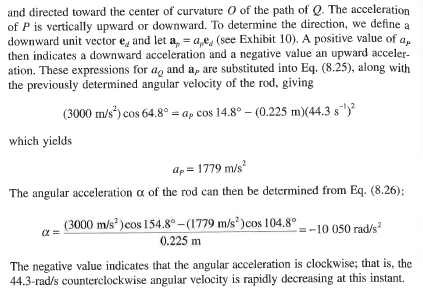
\includegraphics[scale=1.1]{example_8_12b.png}


\end{itemize}
\newpage

	

\end{document}



